\cotefile{157-5}

\scanpage{588}

\deleted{

\handwritten{\diagram{\begin{tikzcd}[ampersand replacement=\&,row sep=0.2em]
\unsure{\mathcal M|M}\mathbin{\overset{\mathrm{Loc}}{\boxtimes}}\unsure{\mathcal N|N}\\
\mathrel{\begin{tikzpicture}[baseline=-0.5ex]\node[rotate=90,inner sep=0pt]{$\simeq$};\end{tikzpicture}}\\
\underline{\mathrm{Hom}}^{!}_{\mathrm{Loc}}(\mathcal M^{\mathrm o},\mathcal N)
\end{tikzcd}}}

\handwritten{\[
\underbrace{\underline{\mathrm{Hom}}_{!\mathrm{Loc}}(\mathcal M,\deleted{\unsure{N}}\unsure{P|\mathcal P})}_{
\left\{\begin{gathered}
\inserted{\text{\unsure{des} }\underline{\mathrm{Hom}}\text{, et }\underline{\mathrm{Hom}}}\\
\text{\unsure{stables} par }\underset{\longrightarrow}{\lim}\\
\text{\unsure{localiseurs} }\inserted{\text{\unsure{Loc}}}\text{\unsure{-stables}}\\[-2pt]
\deleted{\unsure{P}}
\end{gathered}\right.}
\]}

\handwritten{$\boxed{\mathcal M,\mathcal N\quad\text{\unsure{Loc-paratopos|Loc-protopos}}}$

$P$ catégorie stable par p. $\underset{\longrightarrow}{\lim}$, \unsure{avec|un} localiseur \unsure{stable} par lesdites $\underset{\longrightarrow}{\lim}$.}

\handwritten{\[
\underline{\mathrm{Hom}}_{!\mathrm{Loc}}(\mathcal M\boxtimes\mathcal N,P)
\xrightarrow{\approx}\underline{\mathrm{Hom}}_{!\mathrm{Loc}}
(\mathcal M,\underline{\mathrm{Hom}}_{!\mathrm{Loc}}(\mathcal N,P))
\]}

\handwritten{\[
\begin{aligned}
f_i&\longrightarrow g_i\\
f=\underset{\longrightarrow}{\lim}\, f_i&\longrightarrow g=\underset{\longrightarrow}{\lim}\,g_i\\
f(\unsure{x|u})=\underset{\longrightarrow}{\lim}\,f_i(x)&\longrightarrow \begin{tikzpicture}[baseline=(term.base)]
\node[inner sep=0pt,outer sep=0pt] (term) {$\displaystyle g(x)=\underset{\longrightarrow}{\lim}\,g_i(x)$};
\draw[overlay,line width=.35pt]
 ([xshift=1em,yshift=5.4ex]term.north west)
 .. controls +(.05em,-1.8ex) and +(-.12em,.5ex) .. ([xshift=1.35em,yshift=.8ex]term.north west)
 .. controls +(.5em,1.1ex) and +(-1.5em,.4ex) .. ([xshift=-.5em,yshift=.8ex]term.north east)
 .. controls +(1.35em,-.25ex) and +(1.1em,.2ex) .. ([xshift=.16em,yshift=-.4ex]term.south east)
 .. controls +(-1.1em,-.6ex) and +(.8em,.15ex) .. ([xshift=1.2em,yshift=-.6ex]term.south west)
 .. controls +(-.6em,-.15ex) and +(.12em,1.2ex) .. ([xshift=.85em,yshift=-4.0ex]term.south west);
\end{tikzpicture}
\end{aligned}
\]}

\handwritten{\diagram{\begin{tikzcd}[ampersand replacement=\&,row sep=0.1em,column sep=small]
\unsure{f_g|f}(x) \& f(y)\arrow[l]\\
\begin{tikzpicture}[baseline=-0.5ex]\node[rotate=90,inner sep=0pt]{$\simeq$};\end{tikzpicture}
\&\begin{tikzpicture}[baseline=-0.5ex]\node[rotate=90,inner sep=0pt]{$\simeq$};\end{tikzpicture}\\
\underset{\longrightarrow}{\lim}\,f_i(x)\&\underset{\longleftrightarrow}{\lim}\,f_i(y)
\end{tikzcd}}}

\handwritten{Si $\mathcal M$ \deleted{\unsure{et}} et $\mathcal N$ \deleted{ont} des str. de Quillen spéciales, aussi $\mathcal M\mathbin{\overset{\mathrm{Loc}}{\boxtimes}}\mathcal N$ ? et $\underline{\mathrm{Hom}}_{!\mathrm{Loc}}(\mathcal M,N)$ ??}

\handwritten{\[
\mathcal M\mathbin{\overset{\mathrm{Loc}}{\boxtimes}}\deleted{\unsure{\mathcal C}}\widehat I
\mathrel{\overset{\mathrm{Loc}}{\underline{\approx}}}\mathcal M(I)
\qquad C_{\mathcal M}\boxtimes\mathrm{Fl}\,(\widehat I)
\]}

\handwritten{\[
\begin{gathered}
\begin{tikzpicture}[baseline=-0.5ex]\node[rotate=90,inner sep=0pt]{$\simeq$};\end{tikzpicture}\hfill\\[-2pt]
\underline{\mathrm{Hom}}^{!}(\widehat I^{\mathrm o},\mathcal M)
\approx(\underline{\mathrm{Hom}}_{!}(\widehat I,\mathcal M^{\mathrm o}))^{\mathrm o}
\approx(\underline{\mathrm{Hom}}(I,\mathcal M^{\unsure{\mathrm o}}))^{\mathrm o}
\approx\underline{\mathrm{Hom}}(I^{\mathrm o},\mathcal M)
\end{gathered}
\]}

\handwritten{\[
\begin{aligned}
\mathcal M\qquad W&=\mathrm{Is},\quad C\deleted{\unsure{of}}=\mathrm{Mon},\quad F\deleted{\unsure{ib}}=\mathrm{Ep}\ \mathrm{eff}.\\
\mathrm{TC}&=\mathrm{TF}=\mathrm{Is}
\end{aligned}
\]}

\handwritten{\diagram{\begin{tikzcd}[ampersand replacement=\&,row sep=small,column sep=small]
\&\deleted{C}\arrow[r,leftrightarrow] \& \deleted{\mathrm{TC}=\mathrm{Is}}\\
\deleted{\unsure{\mathrm T_y\mathrm F_{\mathrm{inj}}|\mathrm T\mathrm F_{\mathrm{inj}}}}\arrow[ur,dash] \& {}=C_* \arrow[r,leftrightarrow]\arrow[ur,dash,"{\unsure{-|\swarrow}}"'{pos=0.15}] \& F=\mathrm{Fl}
\end{tikzcd}}}

\handwritten{\diagram{\begin{tikzcd}[ampersand replacement=\&,row sep=small,column sep=small]
 C=\mathrm{Fl}^{\unsure{?|\times}}\arrow[r]\arrow[d,dash] \& \mathrm{TC}=\mathrm{Is}\arrow[d,dash]\\
 C_*=\mathrm{Is}=\mathrm{TF} \& F=\mathrm{Fl}\arrow[l]
\end{tikzcd}}}

}

% letterhead
% Printed upside down relative to the handwritten notes.
\noindent\begin{minipage}[t]{.48\linewidth}\raggedright\small
MINISTERE DE L'EDUCATION NATIONALE\\
\unsure{ACADEMIE} D'AIX-MARSEILLE\\
\hspace{2em}\rule{2cm}{0.3pt}\\
\unsure{Inspection} Académique\\
de Vaucluse\\
\hspace{2em}\rule{2cm}{0.3pt}\\
Tél. : 90 82 99 76\\
Référence : Secrétariat n°
\end{minipage}\hfill%
\begin{minipage}[t]{.48\linewidth}\raggedright\small
AVIGNON, le\\
L'Inspecteur d'académie,\\
directeur des services départementaux\\
de l'Education Nationale de Vaucluse,\\
à M
\end{minipage}

% archive sheet number: 587
